\section{Comparison}
\subsection{Comparison with Different Threads per Thread Block}

\subsubsection{Brich3}
\begin{figure}[H]
\centering
\begin{tikzpicture}
\begin{axis}[
    xlabel={Number of Threads},
    ylabel={Execution Duration (seconds)},
    xmin=0.5, xmax=8.5,
    ymin=0..5, ymax=0.7,
    xtick={1, 2, 4, 6, 8},
    ytick={0.656673183, 0.337282581, 0.194313506, 0.123312713, 0.1061290290000 },
    ymajorgrids=true,
    grid style=dashed,
]
\addplot[
    color=orange,
    mark=*,
    ]
    coordinates {
    (1,0.656673183) (2,0.337282581) (4,0.194313506) (6,0.123312713) (8,0.106129029)
    };
\end{axis}
\end{tikzpicture}
\caption{Execution Duration vs. Number of Threads for Birch3}
\label{fig:birch}
\end{figure}

\subsubsection{Circle}
\begin{figure}[H]
\centering
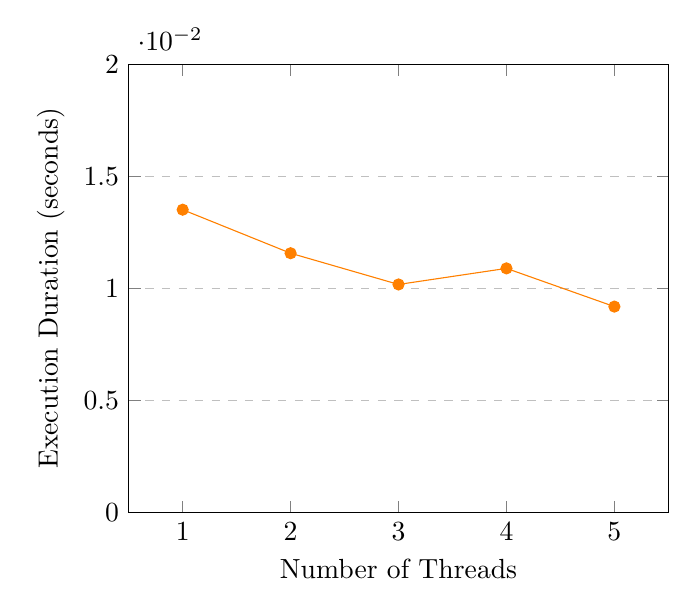
\begin{tikzpicture}
\begin{axis}[
    xlabel={Number of Threads},
    ylabel={Execution Duration (seconds)},
    xmin=0.5, xmax=5.5,
    ymin=0, ymax=0.02,
    xtick={1, 2, 3, 4, 5},
    ytick={0, 0.005, 0.01, 0.015, 0.02},
    ymajorgrids=true,
    grid style=dashed,
]
\addplot[
    color=orange,
    mark=*,
    ]
    coordinates {
    (1,0.013509184) (2,0.011566795) (3,0.010173890) (4,0.010891230) (5,0.009185814)
    };

\end{axis}
\end{tikzpicture}
\caption{Execution Duration vs. Number of Threads for Circle}
\label{fig:circle}
\end{figure}

\subsubsection{Hepta}
% Hepta
\begin{figure}[H]
\centering
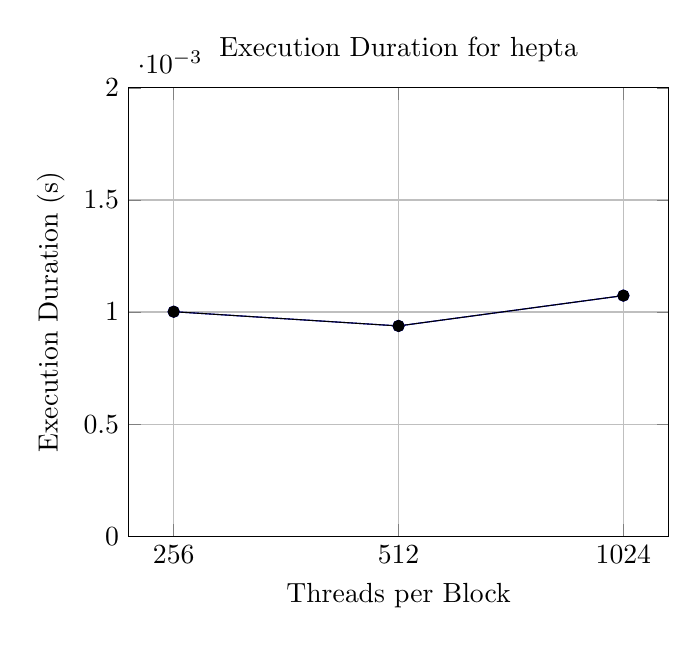
\begin{tikzpicture}
    \begin{axis}[
        xlabel={Threads per Block},
        ylabel={Execution Duration (s)},
        symbolic x coords={256, 512, 1024},
        xtick=data,
        ymin=0, ymax=0.002,
        grid=major,
        title={Execution Duration for hepta}
    ]
        \addplot coordinates {(256,0.00100147) (512,0.000937984) (1024,0.00107334)};
        \addplot[mark=*] coordinates {(256,0.00100147) (512,0.000937984) (1024,0.00107334)};
    \end{axis}
\end{tikzpicture}
\caption{Comparison of execution duration for the dataset Hepta: N212 with different
threads per thread block. Experiments are conducted on an NVIDIA RTX4070 consumer GPU}
\end{figure}

\subsubsection{Isolation}
\begin{figure}[H]
\centering
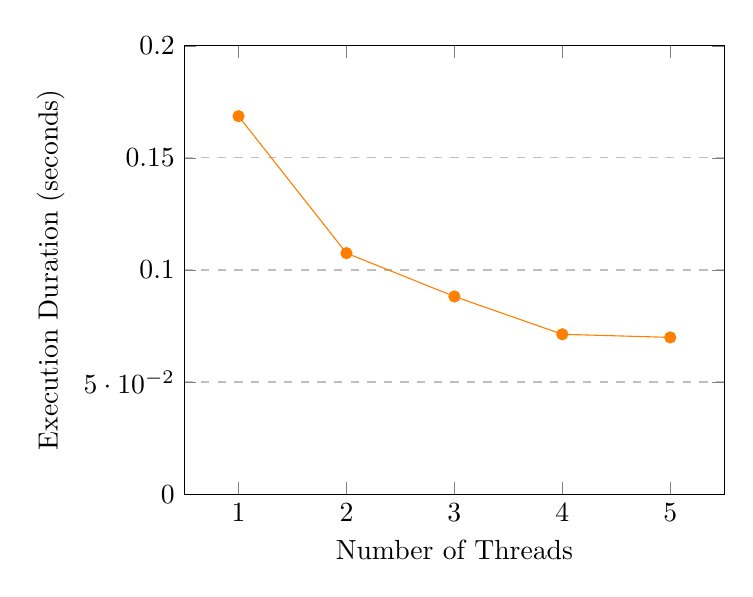
\begin{tikzpicture}
\begin{axis}[
    xlabel={Number of Threads},
    ylabel={Execution Duration (seconds)},
    xmin=0.5, xmax=5.5,
    ymin=0, ymax=0.2,
    xtick={1, 2, 3, 4, 5},
    ytick={0, 0.05, 0.1, 0.15, 0.2},
    ymajorgrids=true,
    grid style=dashed,
]

\addplot[
    color=orange,
    mark=*,
    ]
    coordinates {
    (1,0.168613077) (2,0.107514931) (3,0.088181996) (4,0.071310858) (5,0.069919249)
    };

\end{axis}
\end{tikzpicture}
\caption{Execution Duration vs. Number of Threads for Isolation}
\label{fig:isolation}
\end{figure}

\subsubsection{Smile}
\begin{figure}[H]
\centering
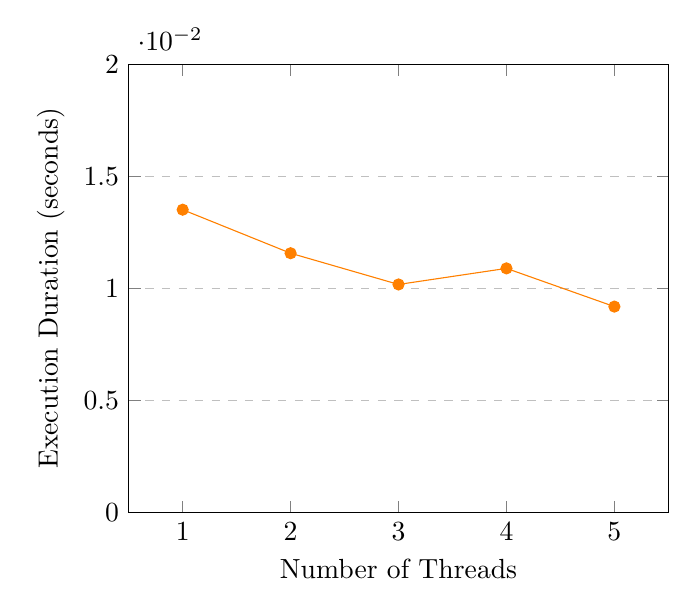
\begin{tikzpicture}
\begin{axis}[
    xlabel={Number of Threads},
    ylabel={Execution Duration (seconds)},
    xmin=0.5, xmax=5.5,
    ymin=0, ymax=0.02,
    xtick={1, 2, 3, 4, 5},
    ytick={0, 0.005, 0.01, 0.015, 0.02},
    ymajorgrids=true,
    grid style=dashed,
]
\addplot[
    color=orange,
    mark=*,
    ]
    coordinates {
    (1,0.013509184) (2,0.011566795) (3,0.010173890) (4,0.010891230) (5,0.009185814)
    };

\end{axis}
\end{tikzpicture}
\caption{Execution Duration vs. Number of Threads for Circle}
\label{fig:circle}
\end{figure}


\subsection{Comparison with Different Methods}

\subsubsection{Brich3}
\begin{figure}[H]
\centering
\begin{tikzpicture}
\begin{axis}[
    xlabel={Number of Threads},
    ylabel={Execution Duration (seconds)},
    xmin=0.5, xmax=8.5,
    ymin=0..5, ymax=0.7,
    xtick={1, 2, 4, 6, 8},
    ytick={0.656673183, 0.337282581, 0.194313506, 0.123312713, 0.1061290290000 },
    ymajorgrids=true,
    grid style=dashed,
]
\addplot[
    color=orange,
    mark=*,
    ]
    coordinates {
    (1,0.656673183) (2,0.337282581) (4,0.194313506) (6,0.123312713) (8,0.106129029)
    };
\end{axis}
\end{tikzpicture}
\caption{Execution Duration vs. Number of Threads for Birch3}
\label{fig:birch}
\end{figure}

\subsubsection{Circle}
\begin{figure}[H]
\centering
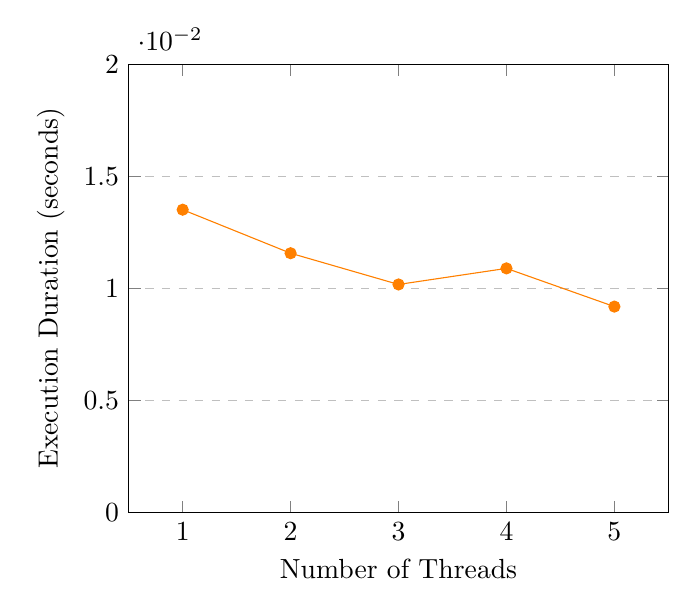
\begin{tikzpicture}
\begin{axis}[
    xlabel={Number of Threads},
    ylabel={Execution Duration (seconds)},
    xmin=0.5, xmax=5.5,
    ymin=0, ymax=0.02,
    xtick={1, 2, 3, 4, 5},
    ytick={0, 0.005, 0.01, 0.015, 0.02},
    ymajorgrids=true,
    grid style=dashed,
]
\addplot[
    color=orange,
    mark=*,
    ]
    coordinates {
    (1,0.013509184) (2,0.011566795) (3,0.010173890) (4,0.010891230) (5,0.009185814)
    };

\end{axis}
\end{tikzpicture}
\caption{Execution Duration vs. Number of Threads for Circle}
\label{fig:circle}
\end{figure}

\subsubsection{Hepta}
% Hepta
\begin{figure}[H]
\centering
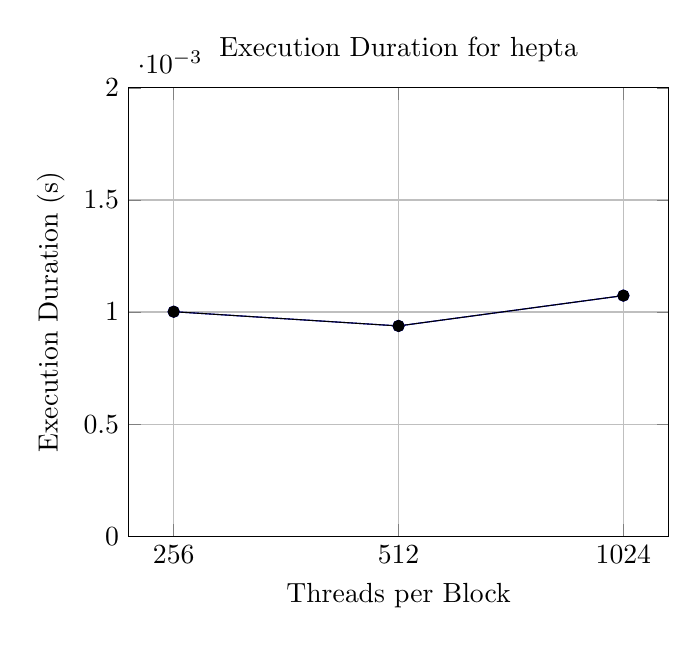
\begin{tikzpicture}
    \begin{axis}[
        xlabel={Threads per Block},
        ylabel={Execution Duration (s)},
        symbolic x coords={256, 512, 1024},
        xtick=data,
        ymin=0, ymax=0.002,
        grid=major,
        title={Execution Duration for hepta}
    ]
        \addplot coordinates {(256,0.00100147) (512,0.000937984) (1024,0.00107334)};
        \addplot[mark=*] coordinates {(256,0.00100147) (512,0.000937984) (1024,0.00107334)};
    \end{axis}
\end{tikzpicture}
\caption{Comparison of execution duration for the dataset Hepta: N212 with different
threads per thread block. Experiments are conducted on an NVIDIA RTX4070 consumer GPU}
\end{figure}

\subsubsection{Isolation}
\begin{figure}[H]
\centering
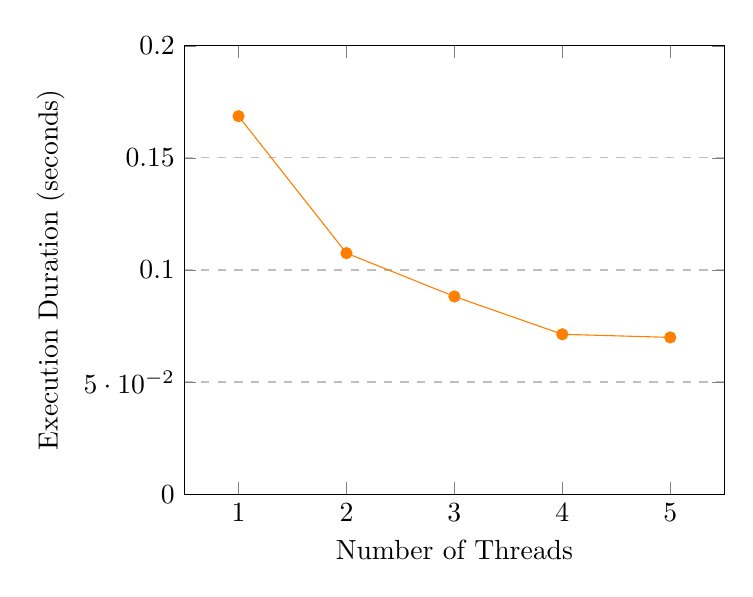
\begin{tikzpicture}
\begin{axis}[
    xlabel={Number of Threads},
    ylabel={Execution Duration (seconds)},
    xmin=0.5, xmax=5.5,
    ymin=0, ymax=0.2,
    xtick={1, 2, 3, 4, 5},
    ytick={0, 0.05, 0.1, 0.15, 0.2},
    ymajorgrids=true,
    grid style=dashed,
]

\addplot[
    color=orange,
    mark=*,
    ]
    coordinates {
    (1,0.168613077) (2,0.107514931) (3,0.088181996) (4,0.071310858) (5,0.069919249)
    };

\end{axis}
\end{tikzpicture}
\caption{Execution Duration vs. Number of Threads for Isolation}
\label{fig:isolation}
\end{figure}

\subsubsection{Smile}
\begin{figure}[H]
\centering
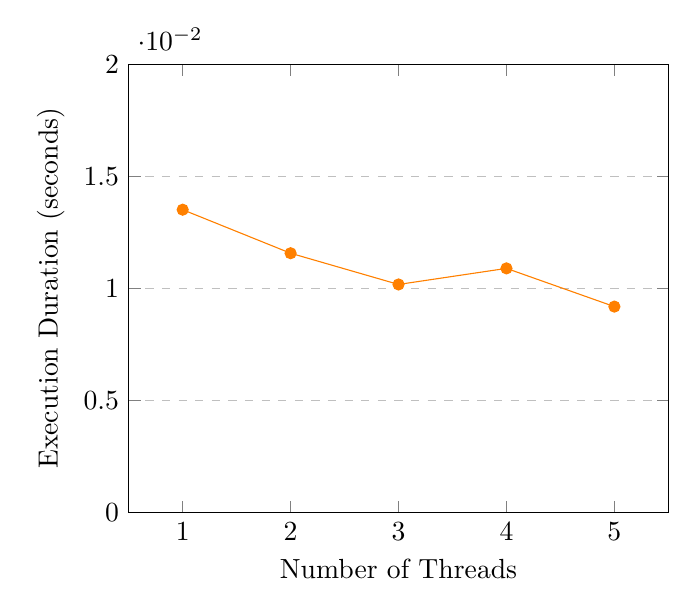
\begin{tikzpicture}
\begin{axis}[
    xlabel={Number of Threads},
    ylabel={Execution Duration (seconds)},
    xmin=0.5, xmax=5.5,
    ymin=0, ymax=0.02,
    xtick={1, 2, 3, 4, 5},
    ytick={0, 0.005, 0.01, 0.015, 0.02},
    ymajorgrids=true,
    grid style=dashed,
]
\addplot[
    color=orange,
    mark=*,
    ]
    coordinates {
    (1,0.013509184) (2,0.011566795) (3,0.010173890) (4,0.010891230) (5,0.009185814)
    };

\end{axis}
\end{tikzpicture}
\caption{Execution Duration vs. Number of Threads for Circle}
\label{fig:circle}
\end{figure}

\subsection{Discussion for different parameter selection and different implementation methods}

In our experiments comparing serial code, OpenMP, and CUDA parallelization, we observed that performance improvements are not always straightforward. The overhead of creating and managing threads sometimes outweighs the benefits of parallelization, especially for smaller tasks. Additionally, imbalanced workloads cause some threads to finish earlier and wait for others, reducing efficiency. Memory access contention, where multiple threads access memory simultaneously, creates bottlenecks. Synchronization points, where threads must wait for each other, also slow down parallel execution. CUDA's performance highly depends on having an optimal configuration and sufficiently large problem sizes; otherwise, the overhead of launching CUDA kernels can make it slower than serial or OpenMP implementations. Understanding these factors is crucial for optimizing parallel computing performance.